% Este archivo es parte de la memoria del proyecto fin de carrera
% de Manuel López Urbina. Protegida bajo la licencia GFDL.
% Para más información, la licencia completa viene incluida en el
% fichero fdl-1.3.tex

% Copyright (C) 2017 Manuel López Urbina


\chapter{Conceptos básicos}
\label{chap:conceptos-básicos}


En el presente capítulo se recogen aquellos conceptos, definiciones, protocolos y diferentes aspectos que resultan de especial interés y que ayudarán a la comprensión de los diferentes puntos tratados en el resto de 
la memoria sin profundizar demasiado en detalles técnicos.\\

Todos estos conceptos se encuentran estrechamente ligados con tecnologías de la comunicación y transmisión de información, más concretamente en el ámbito de la programación web.

\section{Transmisión y comunicación}
\label{sec:transmisión}

Se denomina \emph{transmisión} como el proceso de transporte de una señal de un lugar a otro y \emph{comunicación} como el intercambio entre dos entes mediante una transmisión, los cuales son capaces de
interpretar la información circundante entre ellos y en el cual existen un conjunto de reglas definidas, los protocolos\footnote{Protocolo: reglamento o serie de instrucciones que se fijan por tradición o por convenio. },
que rigen el proceso.


\section{Socket}
\label{sec:def-socket}

\emph{Socket}, o también conocido como conector, designa un concepto abstracto mediante el cual dos programas, generalmente situados en computadoras distintas, pueden intercambiar cualquier flujo de datos
de manera fiable y ordenada.\\

La comunicación a través de una red de ordenadores es una tarea compleja en la que para resolverla se ha empleado un enfoque de diseño por capas, pudiéndose hablar por tanto de una arquitectura 
o pila de protocolos donde cada capa utiliza servicios (funciones) de la capa inferior y ofrece servicios a la capa superior. \\

El modelo de referencia para la comunicación de ordenadores es el denominado modelo de Interconexión de Sistemas Abiertos OSI ( Open Systems Interconection ), el cual queda descrito
en la sección \ref{sec:modelo-osi} junto con la localización de los sockets en dicho modelo.\\

El término \emph{socket} es también usado como el nombre de una interfaz de programación de aplicaciones (API) para la familia de protocolos de red TCP/IP \footnote{ TCP/IP es un conjunto de protocolos que
permiten la comunicación entre los ordenadores pertenecientes a una red. La sigla TCP/IP significa Protocolo de control de transmisión/Protocolo de Internet. Proviene de los nombres de dos protocolos 
importantes incluidos en el conjunto TCP/IP, es decir, del protocolo TCP y del protocolo IP. }, provista usualmente por el sistema operativo.\\

Los sockets constituyen el mecanismo para la entrega de paquetes de datos provenientes de la tarjeta de red a los procesos o hilos apropiados. Un socket queda definido por un par de direcciones IP local
y remota, un protocolo de transporte y un par de números de puerto local y remoto.\\

Cuando se habla de dirección y puerto local/remoto, se sobreentiende que nos referimos a dos procesos (cliente/servidor o nodo/nodo) ya que ambas direcciones IP y puerto pueden coincidir para el intercambio de información entre procesos dentro de una misma máquina
y; además, la comunicación puede ser perfectamente bidireccional, asumiendo que el par que la inicia es el cliente y su contrapartida un servidor pero pudiendo ejercer de forma ambivalente ambas partes.\\


\section{WebSocket}
\label{sec:def-websocket}

Comprendido previamente el concepto de \emph{socket} descrito en el punto \ref{sec:def-socket}, definimos  \emph{Websocket} como una tecnología que proporciona un canal de comunicación bidireccional y full-duplex 
\footnote{Full Duplex: definido como la capacidad de transmisión y recepción en ambas direcciones al mismo tiempo. } utilizada por cualquier aplicación cliente/servidor.\\


La API de WebSocket está siendo normalizada por el W3C, mientras que el protocolo WebSocket ya fue normalizado por la IETF\footnote{Internet Engineering Task Force (IETF) (en español, Grupo de Trabajo de Ingeniería de Internet)
es una organización internacional abierta de normalización, que tiene como objetivos el contribuir a la ingeniería de Internet, actuando en diversas áreas, como transporte, encaminamiento, seguridad.
Se creó en los Estados Unidos, en 1986. Es mundialmente conocido porque se trata de la entidad que regula las propuestas y los estándares de Internet, conocidos como RFC.} como el RFC 6455.\\

Debido a que las conexiones TCP comunes sobre puertos diferentes al 80 son habitualmente bloqueadas por los administradores de redes, el uso de esta tecnología proporcionaría una solución
a este tipo de limitaciones proveyendo una funcionalidad similar a la apertura de varias conexiones en distintos puertos, pero multiplexando diferentes servicios WebSocket sobre un único
puerto TCP a costa de una pequeña sobrecarga del protocolo.



\section{La arquitectura TCP/IP y el modelo OSI}
\label{sec:modelo-osi}

En 1977 la Organización Internacional de Estandarización ( Internacional Standards Organization , ISO) estableció un subcomité encargado de diseñar una arquitectura de
comunicación. El resultado fue el modelo de referencia para la Interconexión de Sistemas Abiertos OSI ( Open Systems Interconection ). Dicho modelo define una arquitectura de
comunicación estructurada en siete niveles verticales. Dicho modelo es utilizado como base teórica para el desarrollo de la arquitectura TCP/IP, la cual está compuesta por una serie de capas
o niveles en los que se encuentran los protocolos que implementan las funciones necesarias para la comunicación entre dos dispositivos en red.\\

Siendo, por tanto, el modelo OSI el empleado en el estudio de las redes de datos y el modelo o arquitectura TCP/IP como un modelo real
empleado es las redes actuales.\\

En la siguiente figura \ref{diagram:modelo-osi-tcp} se aprecian los niveles o capas de los modelos OSI y TCP/IP.\\

\begin{figure}[H]
  \begin{center}
    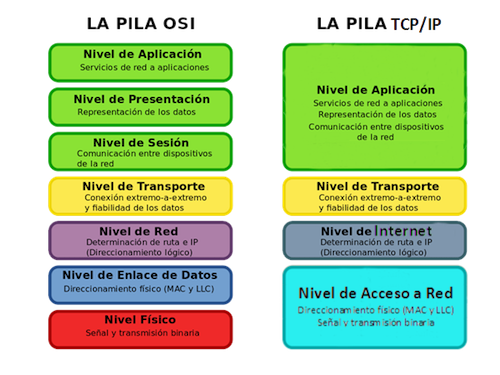
\includegraphics[scale=0.8]{imagenes/osi-tcp.png}
  \end{center}
  \caption{ Representación de capas o niveles OSI y TCP/IP.}
  \label{diagram:modelo-osi-tcp}
\end{figure}

Los sockets dentro del modelo TCP/IP se pueden ver como una interfaz con la capa de transporte.


\begin{figure}[H]
  \begin{center}
    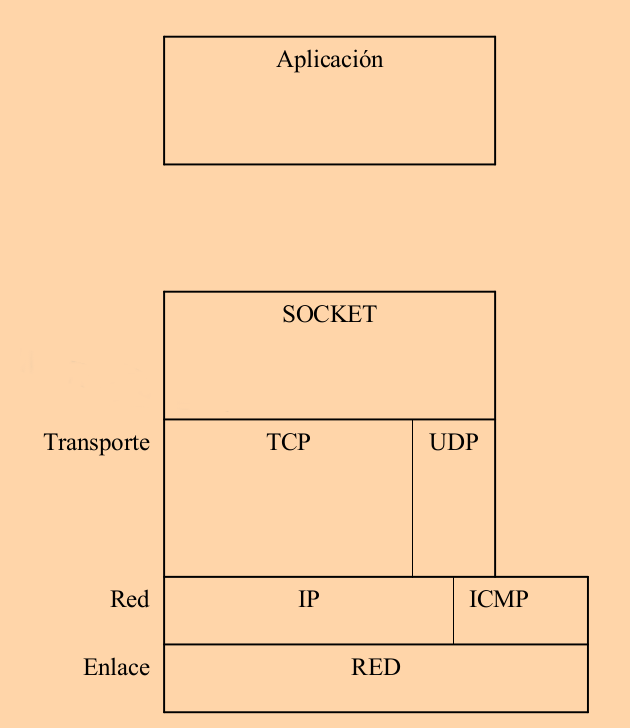
\includegraphics[scale=0.5]{imagenes/modelo-tcp-ip-socket.png}
  \end{center}
  \caption{ Representación de los sockets como una interfaz de la capa de transporte del protocolo TCP/IP.}
  \label{diagram:socket}
\end{figure}


\section{Streaming}
\label{sec:def-streaming}


La retransmisión (en inglés streaming, también denominado transmisión) es la distribución digital de contenido multimedia a través de una red de computadoras, 
de manera que el usuario utiliza el producto a la vez que se es descargado. La palabra retransmisión se refiere a una corriente continua que fluye sin interrupción, habitualmente audio o vídeo, aplicándose la difusión 
de vídeo en el presente proyecto. \\

Este tipo de tecnología funciona mediante un búfer de datos que va almacenando el flujo de descarga en la estación del usuario para inmediatamente mostrarle el material descargado. Esto se contrapone al mecanismo de
descarga de archivos, que requiere que el usuario descargue los archivos por completo para poder acceder al contenido.\\

La retransmisión requiere de una conexión por lo menos de igual ancho de banda que la tasa de transmisión del servicio. La retransmisión de vídeo por Internet se popularizó a fines de la década de 2000, 
cuando la contratación del suficiente ancho de banda para utilizar estos servicios en el hogar se hizo lo suficientemente barato.



\section{Framework}
\label{sec:def-Framework}

Un framework, también denominado entorno de trabajo o marco de trabajo, es un conjunto estandarizado de conceptos, prácticas y criterios para enfocar un tipo de problemática particular que sirve como
referencia, para enfrentar y resolver nuevos problemas de índole similar.\\

Aplicado a informática, concretamente al desarrollo de software, un entorno de trabajo o framework es una estructura conceptual y tecnológica de asistencia definida, normalmente, con artefactos o 
módulos concretos de software, que puede servir de base para la organización y desarrollo software. Típicamente, puede incluir soporte de programas, bibliotecas, y un lenguaje interpretado, entre 
otras herramientas, para así ayudar a desarrollar y unir los diferentes componentes de un proyecto.\\

En  general,  con  el  término  framework, nos estamos refiriendo a una estructura software compuesta de componentes personalizables e intercambiables para el
desarrollo de una aplicación. En otras palabras, un framework se puede considerar como una aplicación genérica incompleta y configurable a la que podemos añadirle las últimas 
piezas para construir una aplicación concreta.\\

Los objetivos principales que persigue un framework son:

\begin{itemize}
 \item Acelerar el proceso de desarrollo
 \item Reutilización de código.
 \item Promover buenas prácticas de desarrollo como el uso de patrones.
\end{itemize}

